\newpage
\section*{Introduction}

The set of cells contained within this library are based upon $0.35\mu m$ unified CMOS technology. The follow a two-layer metal design on top of a p-type substrate with N-Well and P-Well regions for pull-up and pull-down networks respectively. All cells are a common $17.2\mu m$ high, with varied widths all integer multiples of 1.2µm. 
All transistors are fixed at $W_P = 2.4\mu m$, $L_P = 0.35\mu m$, $W_N = 1.5\mu m$, $L_N = 0.35\mu m$.


Global signals and power rails are arranged horizontally in \textit{metal1}.
Figure \ref{fig:globalsignals} shows this arrangement with the dimensions of the global signals.
While cell I/O signals are arranged vertically in \textit{metal2} and aligned to a $1.2\mu m$ grid.
Power rails are $1.25\mu m$ wide, while other horizontal signals are $0.5\mu m$ wide. 
The distance between horizontal signals is $0.8\mu m$ from centre to centre. 
Both rails are formed using a continuous ohmic region and line of taps. 

\begin{figure}[htb!]
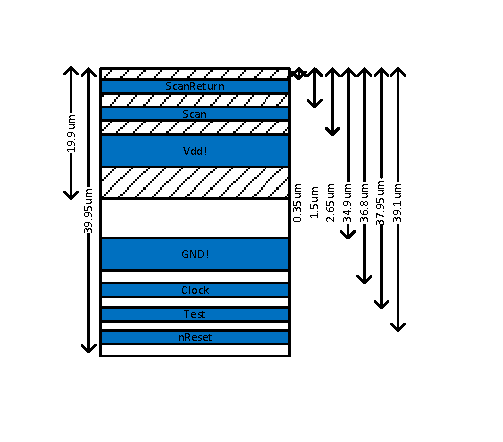
\includegraphics[width=\textwidth]{cellglobals.pdf}
\caption{Global signals common to all cells}
\label{fig:globalsignals}
\end{figure}

Vertical signals lines are $0.6\mu m$ wide with position of each signal measured from the left edge of the cell to the right edge of the metal strip and detailed on each cell page. 

AC characteristics of cells are measured as the propagation delay from each input to each output under normal operation conditions. 
This is set as having each input driven through one inverter and each output loaded by two inverters from this library. 
Each cell lists both the delay to correct output as a result of an input going high, as well as an input going low. 

Major cells in the library have additional sections detailing the stick diagram and transistor layout of each cell as designed by the designated team member. 
Even though only 4 members were in the group, both the half adder and XOR2 have been included in the library and detailed. 
